
\begin{equation}
    \vec{B} - \vec{A} = \myvec{4\\2\\6}, \vec{C} - \vec{A} = \myvec{10\\5\\15}
\end{equation}

Forming the matrix 
\begin{align}
    \vec{M} &= \begin{pmatrix}
    \vec{B} - \vec{A} & \vec{C} - \vec{A}\\
    \end{pmatrix}^\top\\
    &= \begin{pmatrix}
    4 & 2 & 6\\
    10 & 5 & 15
    \end{pmatrix}
\end{align}

Using matrix transformation,
\begin{align}
\vec{M} = \begin{pmatrix}
    4 & 2 & 6\\
    10 & 5 & 15
    \end{pmatrix} \xleftrightarrow{\text{$R_2$}\rightarrow{\text{$R_2 - \dfrac{5}{2} R_1$ }}}
 \begin{pmatrix}
 4 & 2 & 6\\
 0 & 0 & 0
 \end{pmatrix}
\end{align}
 
\begin{equation}
   \implies rank(\vec{M}) = 1 
\end{equation}

Thus $\vec{A}$, $\vec{B}$ and $\vec{C}$ are collinear. 

Let $\vec{B}$ divide AC in the ratio $\lambda$ : 1. 

\begin{align}
    \implies \dfrac{\lambda}{1} &= \dfrac{AB}{BC}\\
    \implies \norm{\vec{B} - \vec{A}} &= \lambda\; \norm{\vec{C} - \vec{B}}
\end{align}
\begin{equation}
    \implies \lambda = \dfrac{2}{3}
\end{equation}
%
Thus $\vec{B}$ divides AC in the ratio 2:3.  See Fig.          \ref{aug/2/13/plot}
% 
\begin{figure}[!h]
    \centering
         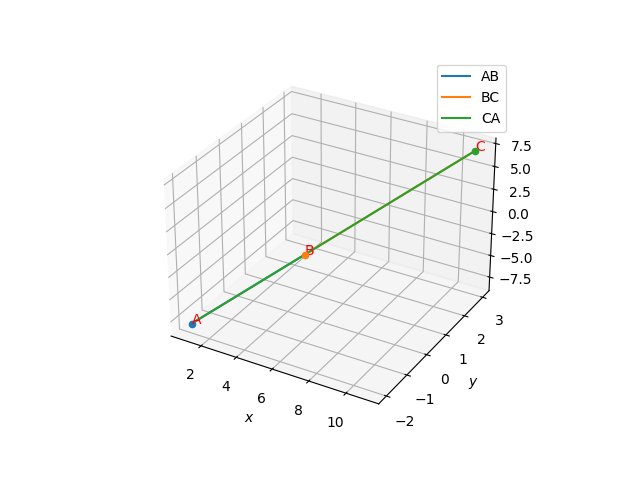
\includegraphics[width=\columnwidth]{solutions/aug/2/13/figures/figure.png}
         \caption{Plot of the line}
         \label{aug/2/13/plot}
\end{figure}

